\section{Experiments}
\label{sec:exps}

\subsection{Agent settings}
All LLM API calls are implemented using the \texttt{Litellm} package \cite{litellm}. 
We evaluated four large language models: \gptmini, \gptmodel, \ofourmodel, and \claudesonnet. 
The user simulator is implemented using \gptmodel.
Each task is run four times, maintaining a consistent LLM temperature of 0 to promote deterministic outputs.
Both the agents and the user simulator are implemented as function-calling agents. All tools are provided to LLMs in the OpenAI tools format.
The agent prompt includes generic guidelines along with domain-specific policies. Similarly, the user prompt contains generic guidelines supplemented by task-specific instructions. Both domain policies and prompts are available in \Cref{app:domain-policies,app:prompts}.

When the \gptmodel agent is paired with the \gptmodel user simulator, the average agent/user simulation costs are \$0.086/\$0.059 per task, respectively.
The cost of running all domains for 1 trial per task is approximately \$40.

\subsection{Results}

\paragraph{Pass\textasciicircum k scores.}

\begin{figure}[t]
    \centering
    \begin{subfigure}[tb]{0.48\textwidth}
        \centering
        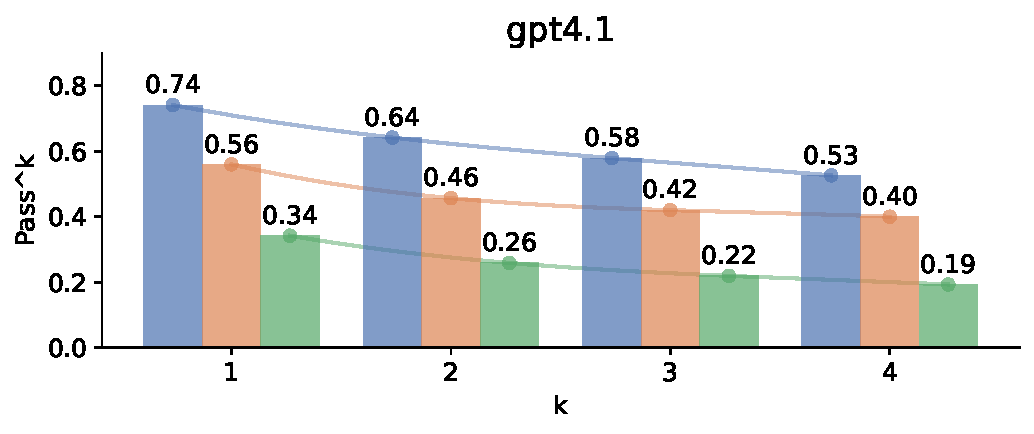
\includegraphics[width=\textwidth]{figures/results/pass_k_metrics_default_all_domains_gpt-4.1-2025-04-14.pdf}
    \end{subfigure}%
    \hfill
    \begin{subfigure}[tb]{0.48\textwidth}
        \centering
        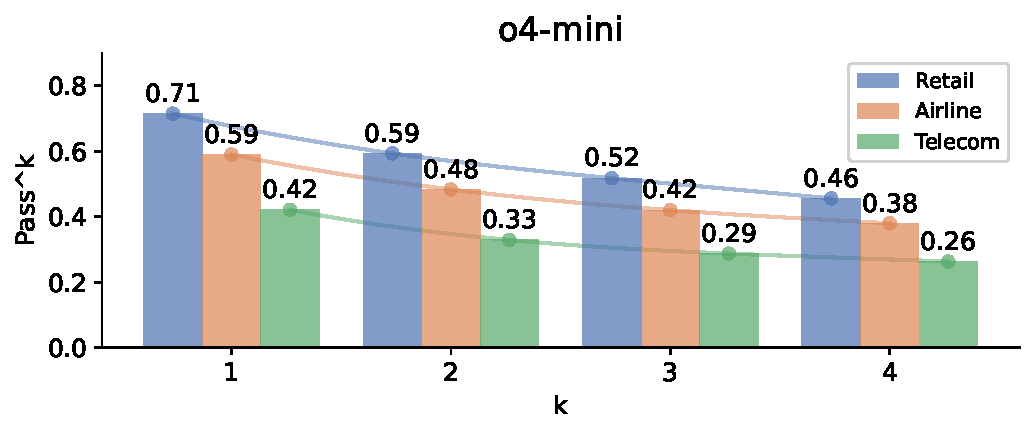
\includegraphics[width=\textwidth]{figures/results/pass_k_metrics_default_all_domains_o4-mini-2025-04-16.pdf}
    \end{subfigure}
    \vspace{1em}
    \begin{subfigure}[tb]{0.48\textwidth}
        \centering
        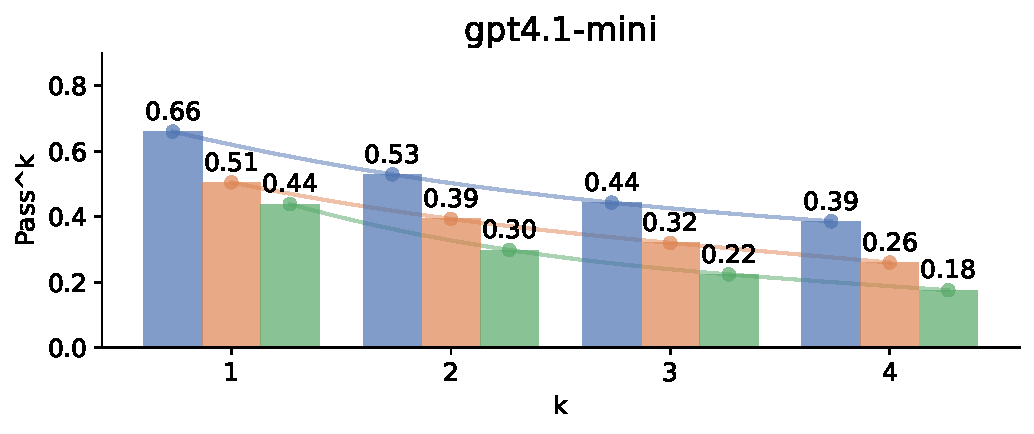
\includegraphics[width=\textwidth]{figures/results/pass_k_metrics_default_all_domains_gpt-4.1-mini-2025-04-14.pdf}
    \end{subfigure}%
    \hfill
    \begin{subfigure}[tb]{0.48\textwidth}
        \centering
        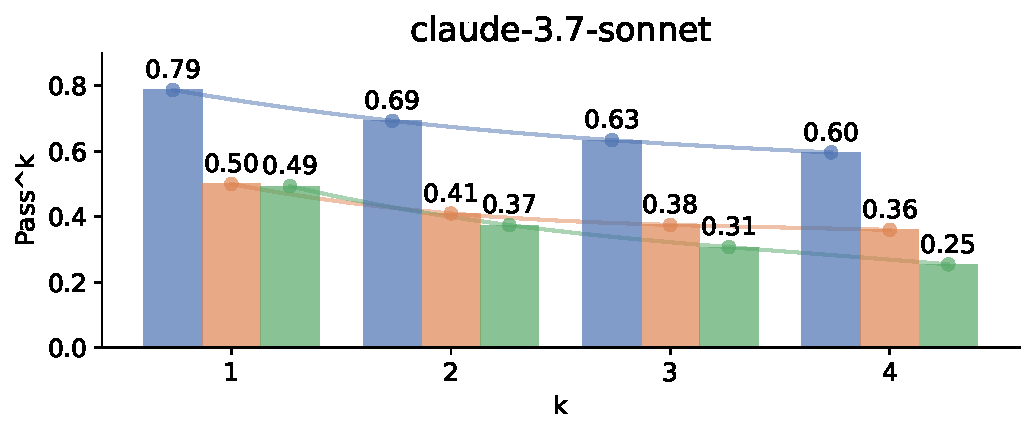
\includegraphics[width=\textwidth]{figures/results/pass_k_metrics_default_all_domains_claude-3-7-sonnet-20250219.pdf}
    \end{subfigure}
    \vspace{-1em}
    \caption{\passk metrics across all evaluated domains (\airline, \retail, \telecom). \textbf{Top Left}: \gptmodelshort, \textbf{Top Right}: \ofourmodelshort, \textbf{Bottom Left}: \gptminishort, \textbf{Bottom Right}: \claudesonnetshort.}
    \label{fig:default_all_domains}
\end{figure}


We computed performance metrics on the verified \bench domains (\retail and \airline) and on our new \telecom domain (see \Cref{fig:default_all_domains}).
Our findings indicate that the \telecom domain presents a greater challenge, exhibiting an overall lower success rate compared to other domains. \gptmodelshort \passone drops from 74\%/56\% for \retail and \airline respectively to 34\% for \telecom.
\gptminishort, \ofourmodelshort, and \claudesonnetshort perform better with \passone of around 50\% for \telecom.
In the case of \claudesonnetshort, the \passone score for \telecom (49\%) is on par with \airline. However, as k increases, the \passk scores decline more rapidly for \telecom compared to \airline, suggesting less consistent performance on the \telecom domain.

\paragraph{Ablation analysis.}

An agent's success in \bench depends on two things -- 1) how well it can communicate and collaborate with the user at solving the issue, and 2) how well it can reason over and apply the domain guidelines specified in the policy document. In order to understand the impact of each of these components—reasoning and communication for dual control—we perform an ablation study. Specifically, we evaluate performance in the \telecom domain across three distinct settings:

\begin{itemize}
    \setlength\itemsep{0em}
    \item \textbf{\basemode}: The default agent and user simulator configuration where the agent and user collaborate in a \textit{dual-control} setup.
    \item \textbf{\solomode}: The agent is provided with a ticket summarizing the user's problem and success criteria. The agent controls all tools, including those typically operated by the user, and is solely responsible for solving the problem. This setting tests the agent's reasoning and tool-calling capability independently of its capacity to interact with the user.
    \item \textbf{\gtmode}: The agent is provided with the sequence of tool calls required to solve the problem, encompassing actions for both the agent and the user. This setup alleviates the agent's reasoning load, focusing on its ability to collaborate with the user to execute a known plan.
\end{itemize}


\Cref{fig:telecom_avg_bar} (left) reports performance across these settings for \gptmodelshort and \ofourmodelshort, revealing key insights. 
The difference between \gtmode and \basemode configurations highlights the impact of the reasoning load on agent performance. 
Unsurprisingly, providing the ground truth leads to better performance than the \basemode setting. But it is notable that this effect is larger for the \ofourmodelshort than for \gptmodelshort, suggesting that \ofourmodelshort is better able to make use of the ground truth information.

\begin{figure}[tb]
    \centering
    \begin{minipage}[t]{0.48\textwidth}
        \centering
        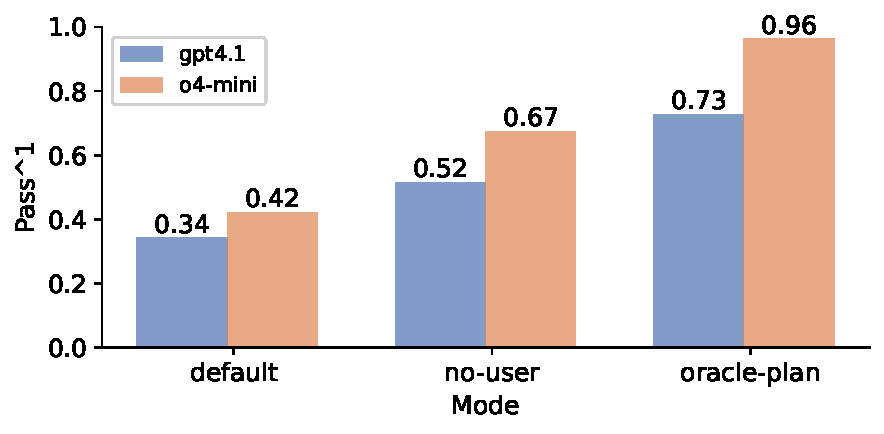
\includegraphics[width=\linewidth]{figures/results/pass_one_metrics_telecom_bar.pdf}
    \end{minipage}
    \hfill
    \begin{minipage}[t]{0.48\textwidth}
        \centering
        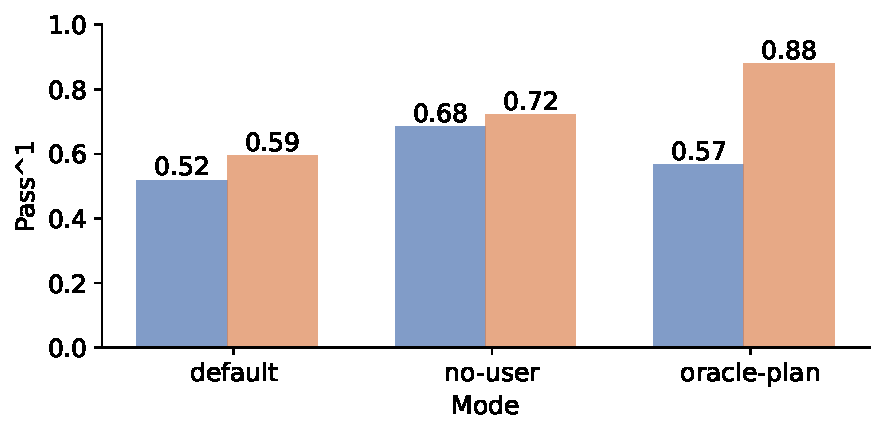
\includegraphics[width=\linewidth]{figures/results/pass_one_metrics_telecom-workflow_bar.pdf}
        \vspace{-1.5em}
    \end{minipage}
    \caption{\passone metrics for the Telecom domain across different operational modes (\basemode, \solomode, \gtmode) using the \basemode user simulation. \textbf{Left}: original policy. \textbf{Right}: workflow-based policy. This figure illustrates the impact of reasoning load and decentralized control on agent performance.}
    \label{fig:telecom_avg_bar}
\end{figure}


The comparison between \solomode and \basemode modes illustrates the impact of dual control and the associated communication overhead on agent error rates and overall success. For both models, shifting from no user operation (\solomode) to a collaborative setup (\basemode) where the agent must guide the user results in a substantial drop in \passone (18\% drop for \gptmodelshort and 25\% drop for \ofourmodelshort).
This underscores that LLMs still face significant challenges when solving problems with an active user who shares control of the environment.

\paragraph{Impact of policy document on performance.}
Figure~\ref{fig:telecom_avg_bar} also allows us to analyze the impact of the policy document on task success. Specifically, we created an alternate policy document that provides more specific details on the workflow required to solve each type of task, with the rationale that having the workflow provides more concrete guidance to the agent (see \Cref{app:technical-support-policy,app:technical-support-policy-workflow}). We observe that this is indeed the case and slightly improves agent performance using the workflow policy (right) over the original one (left) under the \basemode and \solomode modes. Surprisingly, workflow policy document hurts performance on \gtmode for both \gptmodelshort and \ofourmodelshort. Our hypothesis here is that since the agent already has the ground truth action sequence, providing it the workflow might lead to confusion and hurt its performance rather than help.
 
\paragraph{Impact of number of actions and sub-tasks.}




\begin{figure}
    \centering
    \begin{subfigure}[tb]{0.48\textwidth}
        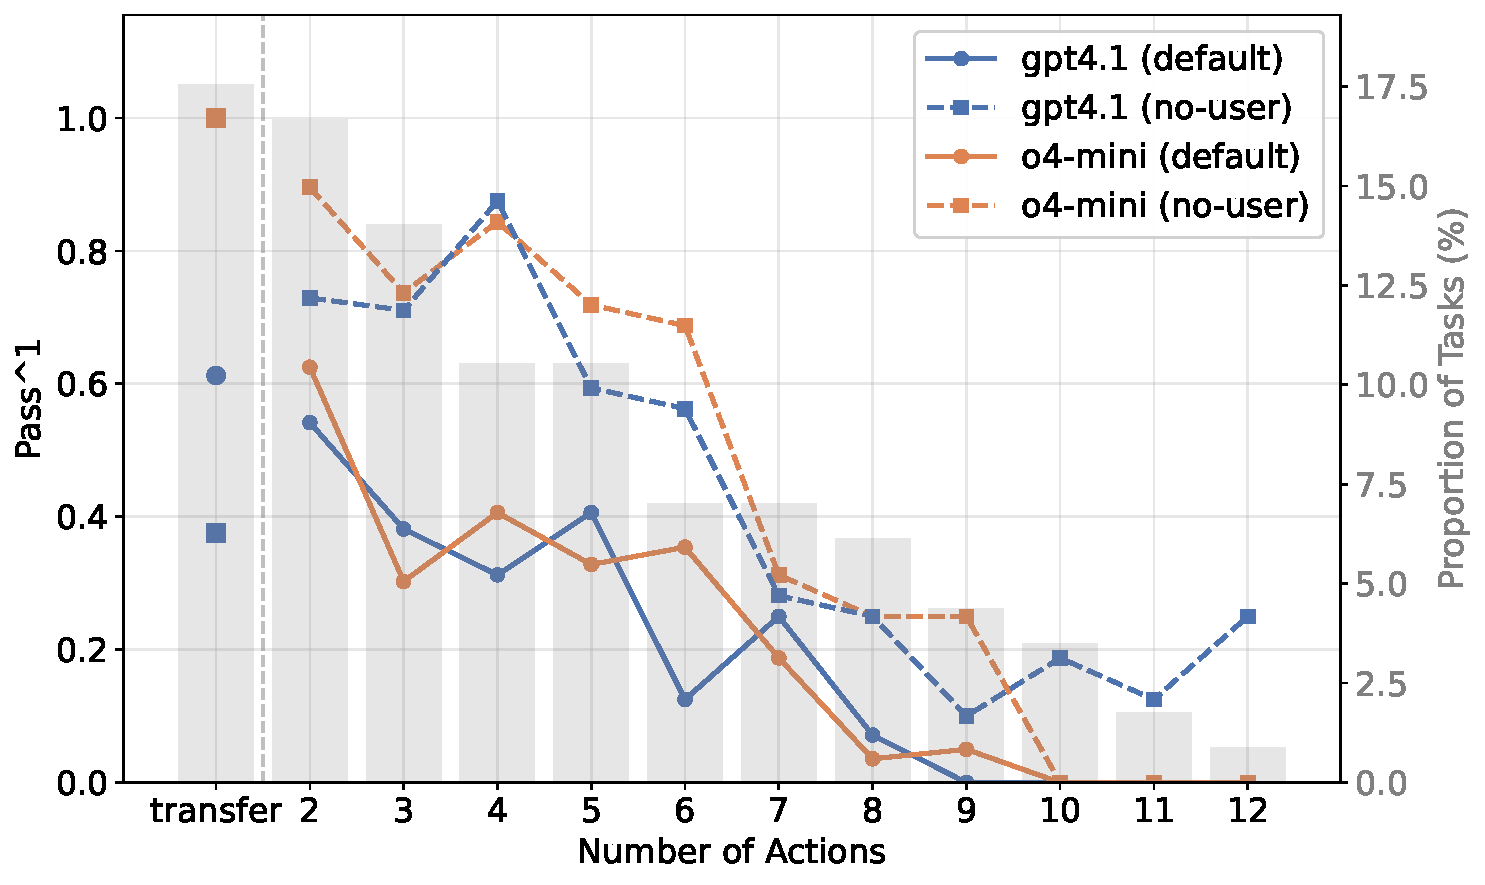
\includegraphics[width=\textwidth]{figures/results/pass_k_vs_num_actions_telecom_all_modes_llm_comparison.pdf}
    \end{subfigure}
    \hfill
    \begin{subfigure}[tb]{0.48\textwidth}
        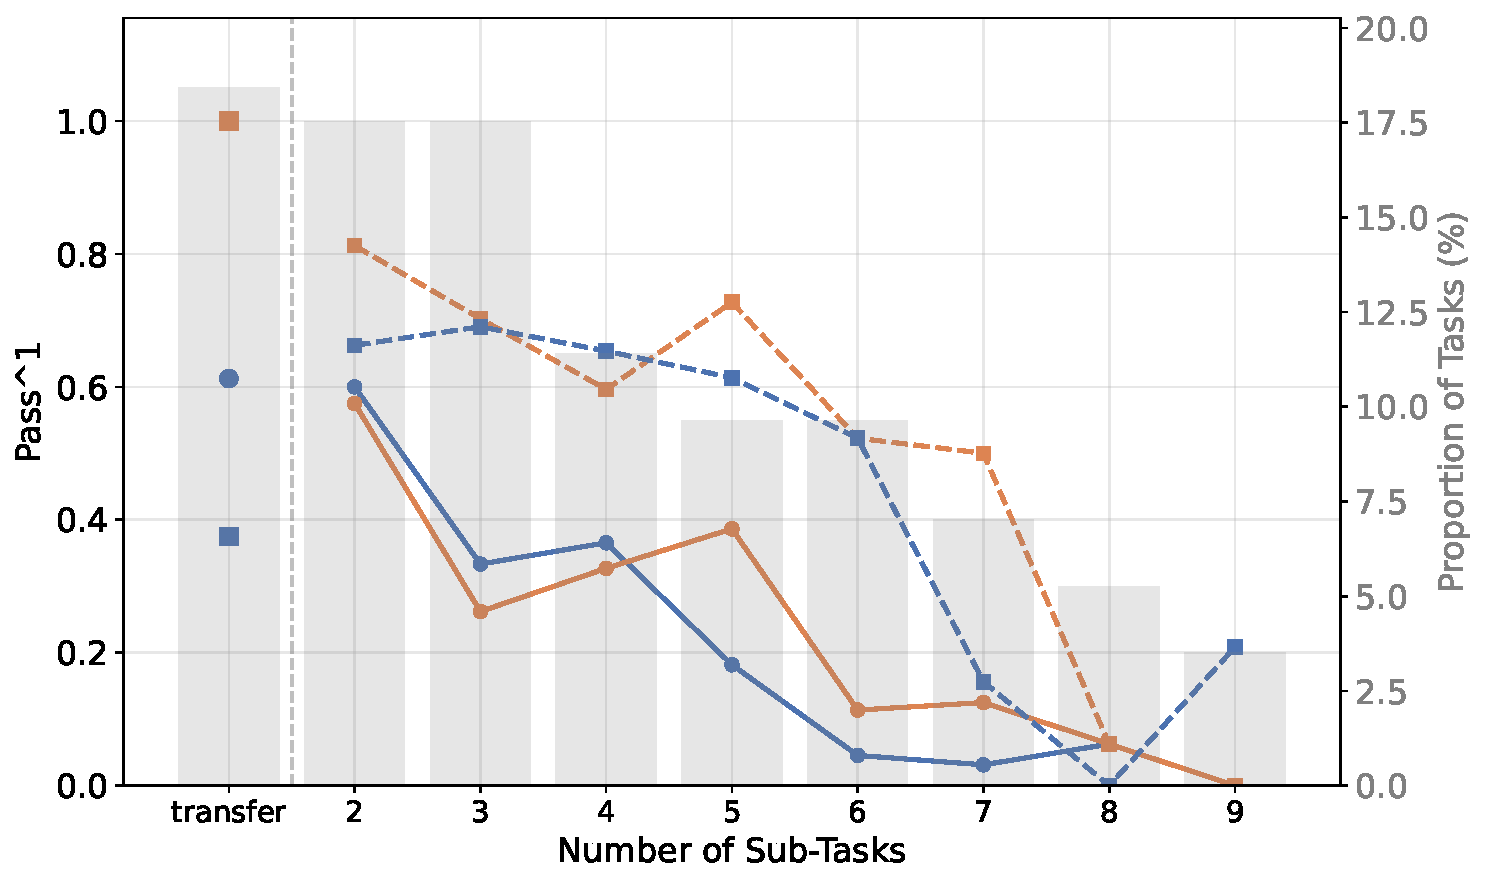
\includegraphics[width=\textwidth]{figures/results/pass_k_vs_num_issues_telecom_all_modes_llm_comparison.pdf}
    \end{subfigure}
    \vspace{-0.5em}
    \caption{\passone scores across various tasks in \telecom binned by the number of actions required to solve them (left) or the number of different issues that need to be addressed (right). \textit{transfer} refers to the special case of a task that requires to be transferred to a human and cannot be solved by the agent alone. (Grey bars indicates the proportion of the tasks that fall into that bin.)}
    \label{fig:telecom_results}
\end{figure}




Figure~\ref{fig:telecom_results} breaks down the \passone  scores across various tasks in \telecom binned by the number of actions required to solve them (left) or the number of different sub-tasks that need to be addressed (right). \textit{transfer} refers to the special case of a task that requires to be transferred to a human and cannot be solved by the agent alone. 

As expected, regardless of the base model being \gptmodelshort or \ofourmodelshort, agent performance drops as the number of actions increases, reaching close to zero for $>7$ actions in \basemode mode. The \solomode mode results in higher scores overall, although the gap reduces (from about 0.3-0.4 to <0.2) as the number of actions increases. This hints that maintaining reliability over longer-horizon tasks remains a challenge under both settings and communication with the user is not the only bottleneck. Interestingly, for \solomode, \gptmodelshort performs better at the tail end (10 actions or more) than \ofourmodelshort.

We observe a similar trend with increase in the number of distinct sub-tasks per task -- performance trends downwards for both base models, with the \texttt{no-user} mode generally being higher than the \texttt{default} mode. Both these results validate that our domain design and task creation process provide a natural path to scaling complexity via increasing action length or combining different sub-tasks into a single task.


\textbf{Impact of issue types.}
The \telecom domain is organized around three primary user intents reflecting the three different issues that can be encountered: \serviceissue, \mobiledataissue, and \mmsissue, each of which contains specific procedures laid out by the domain policy.
These issue types are designed to have an inherent difficulty hierarchy. For instance, \serviceissue tasks can typically be resolved independently through a straightforward sequence of actions.  In contrast, successfully addressing \mobiledataissue or \mmsissue often requires first checking for and potentially resolving underlying \serviceissue problems.  This dependency creates a natural ordering in task difficulty, with \serviceissue being the easiest, while \mobiledataissue and \mmsissue represent more complex, multi-stage problems.

\begin{figure}[tb]
    \centering
    \begin{subfigure}[tb]{0.48\textwidth}
        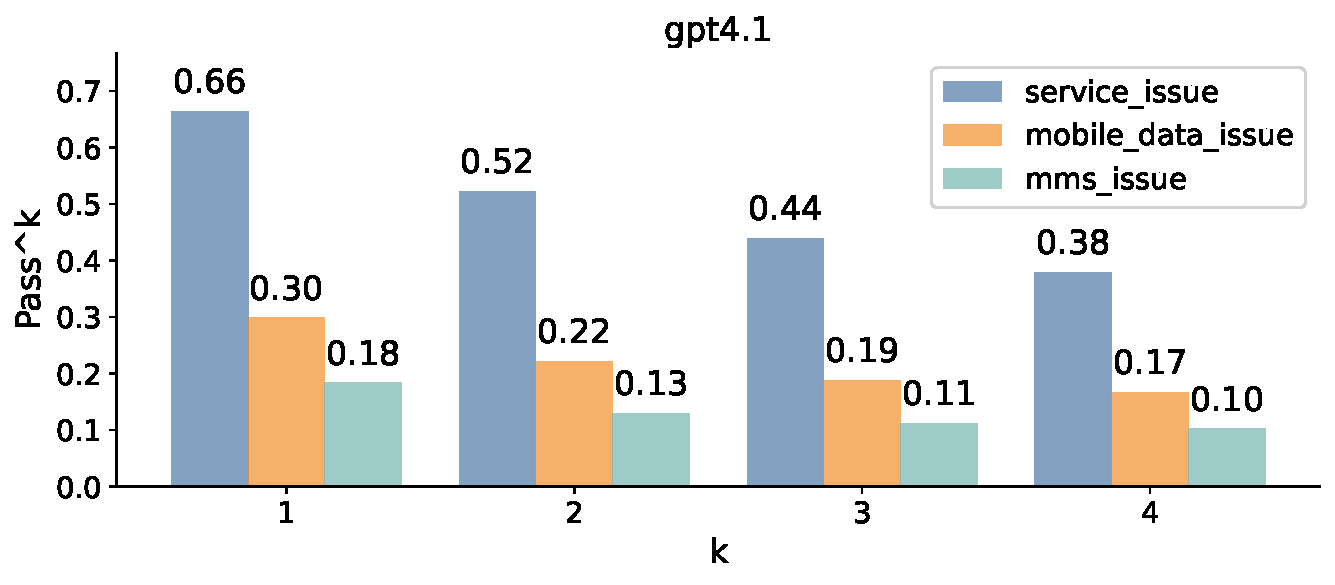
\includegraphics[width=\textwidth]{figures/results/pass_k_vs_k_per_intent_telecom_gpt-4.1-2025-04-14.pdf}
    \end{subfigure}
    \hfill
    \begin{subfigure}[tb]{0.48\textwidth}
        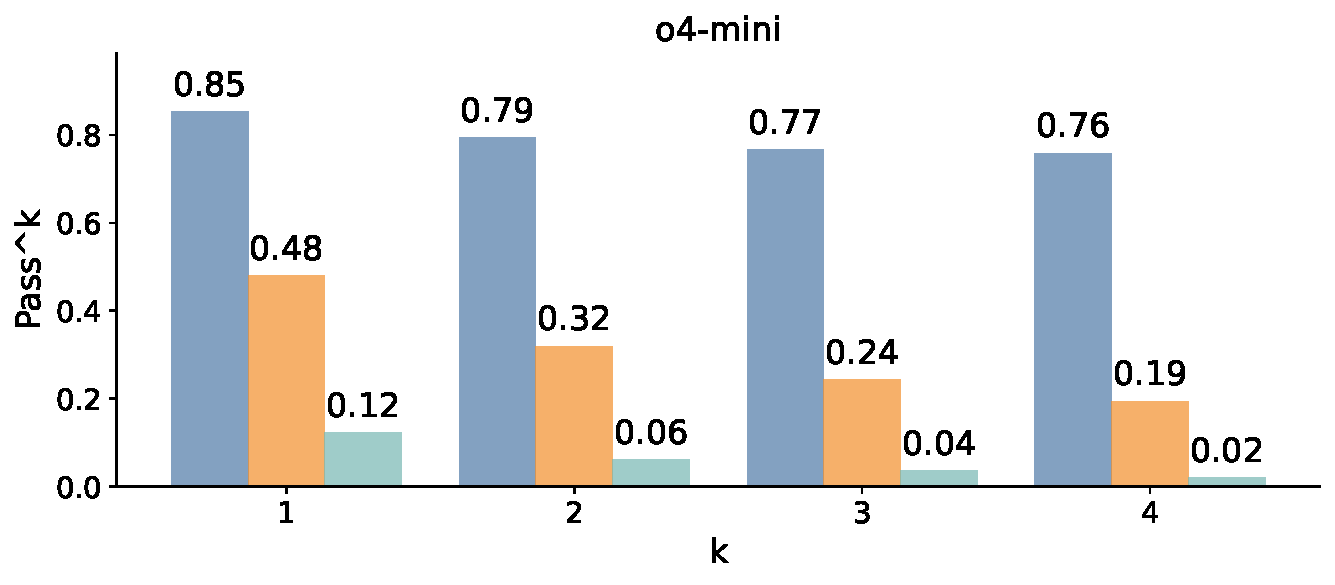
\includegraphics[width=\textwidth]{figures/results/pass_k_vs_k_per_intent_telecom_o4-mini-2025-04-16.pdf}
    \end{subfigure}
    \vspace{0.5em}
    \begin{subfigure}[tb]{0.48\textwidth}
        \centering
        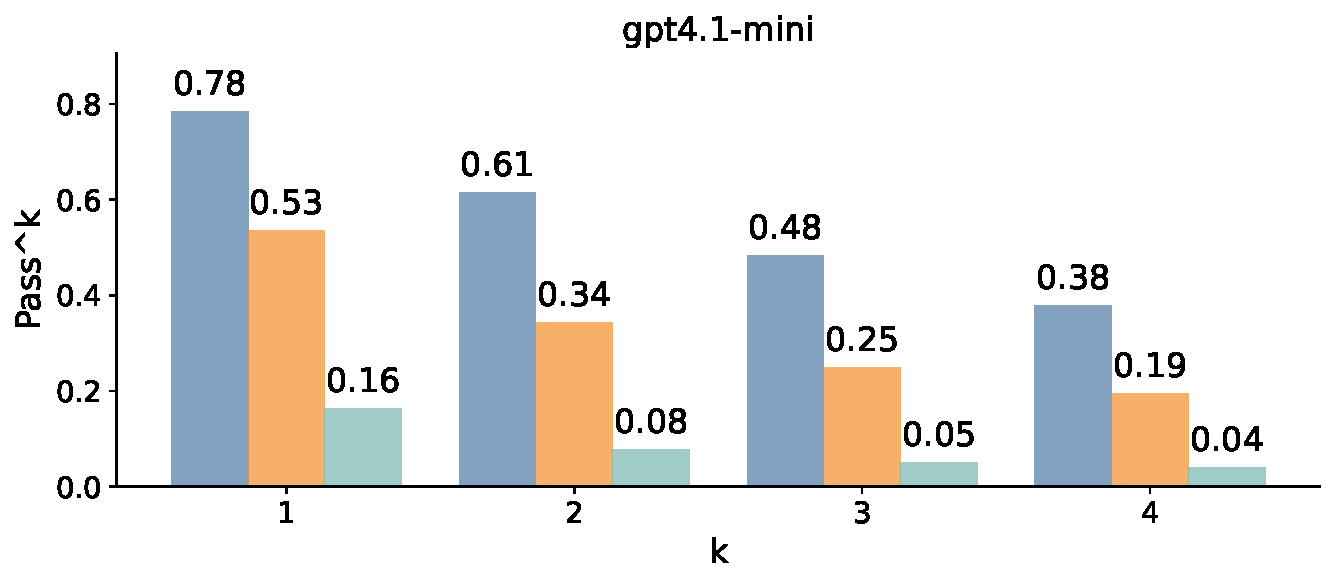
\includegraphics[width=\textwidth]{figures/results/pass_k_vs_k_per_intent_telecom_gpt-4.1-mini-2025-04-14.pdf}
    \end{subfigure}
    \hfill
    \begin{subfigure}[tb]{0.48\textwidth}
        \centering
        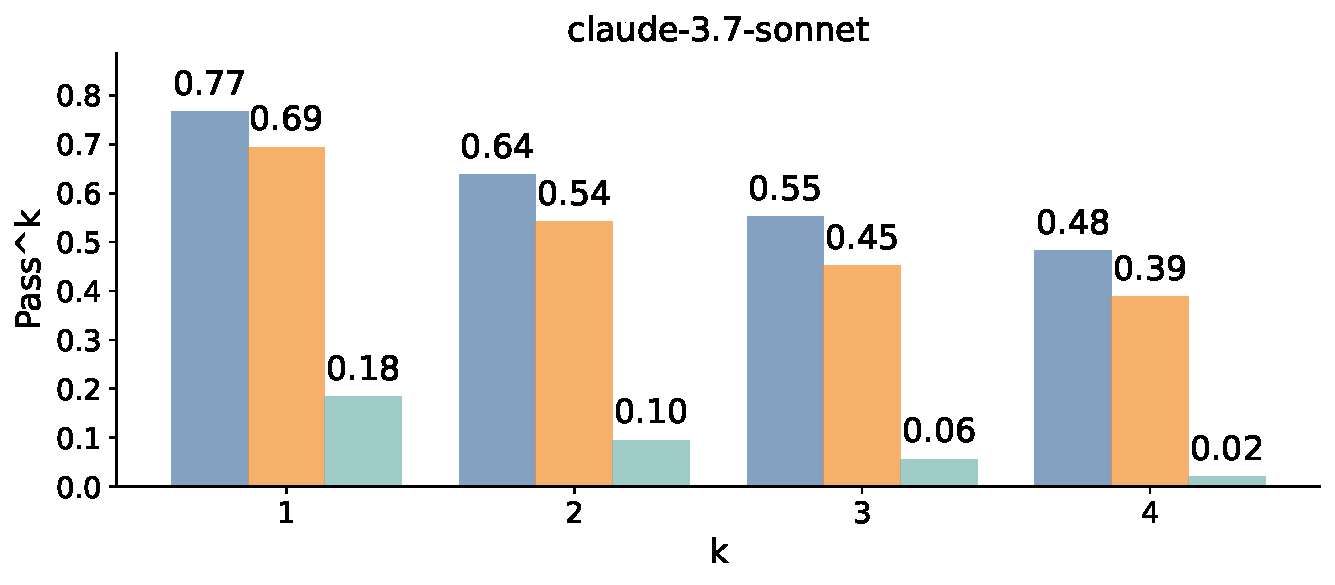
\includegraphics[width=\textwidth]{figures/results/pass_k_vs_k_per_intent_telecom_claude-3-7-sonnet-20250219.pdf}
    \end{subfigure}
    \vspace{-0.8em}
    \caption{\gptmodelshort (top left), \ofourmodelshort (top right), \gptminishort (bottom left), and \claudesonnetshort (bottom right) \passk per issue type for the \telecom domain. Performance is shown for \serviceissue, \mobiledataissue, and \mmsissue issue types, highlighting how different issue types affect success rates.}
    \label{fig:telecom_intent_results}
    \vspace{-1em}
\end{figure}

    


\Cref{fig:telecom_intent_results} provides an breakdown analysis of performance by issue type. We observe that the \passk scores for all LLMs (\gptmodelshort, \ofourmodelshort, \claudesonnetshort, \gptminishort) are driven by higher failure rates on more complex issue types (\mobiledataissue and \mmsissue). This suggests that the multi-stage reasoning and conditional logic required for harder issue types pose a substantial challenge to the agents. We also notice that the spread across issue types differs slightly by the model. For instance, \claudesonnetshort does better than \ofourmodelshort on \mobiledataissue but worse on \serviceissue.

\begin{figure}[tb]
    \centering
    \begin{subfigure}[tb]{0.48\textwidth}
        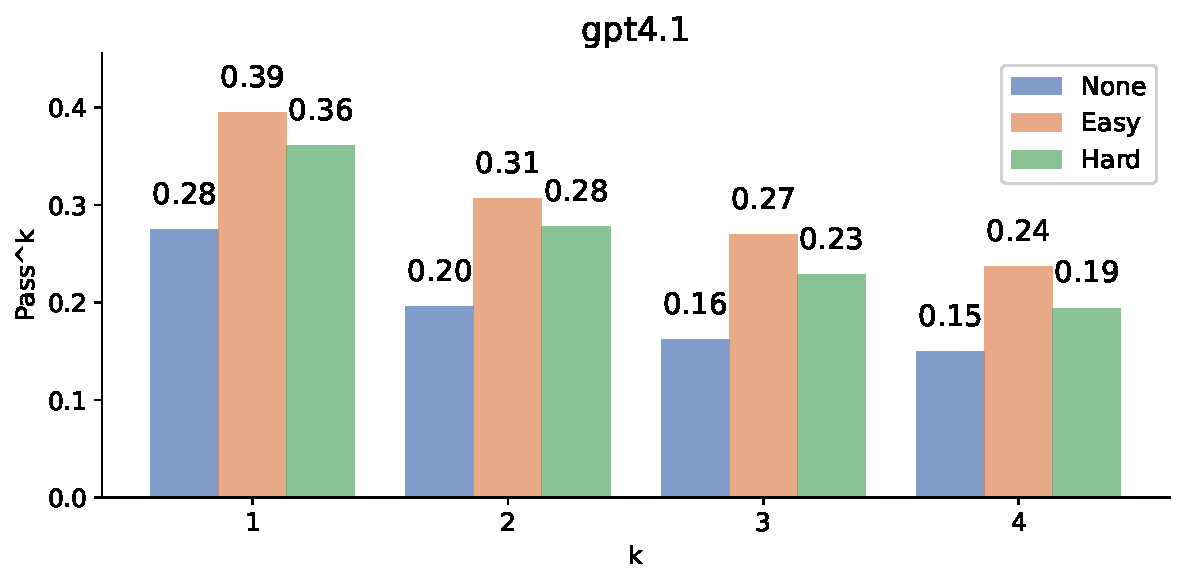
\includegraphics[width=\textwidth]{figures/results/pass_k_vs_k_per_persona_telecom_gpt-4.1-2025-04-14.pdf}
    \end{subfigure}
    \hfill
    \begin{subfigure}[tb]{0.48\textwidth}
        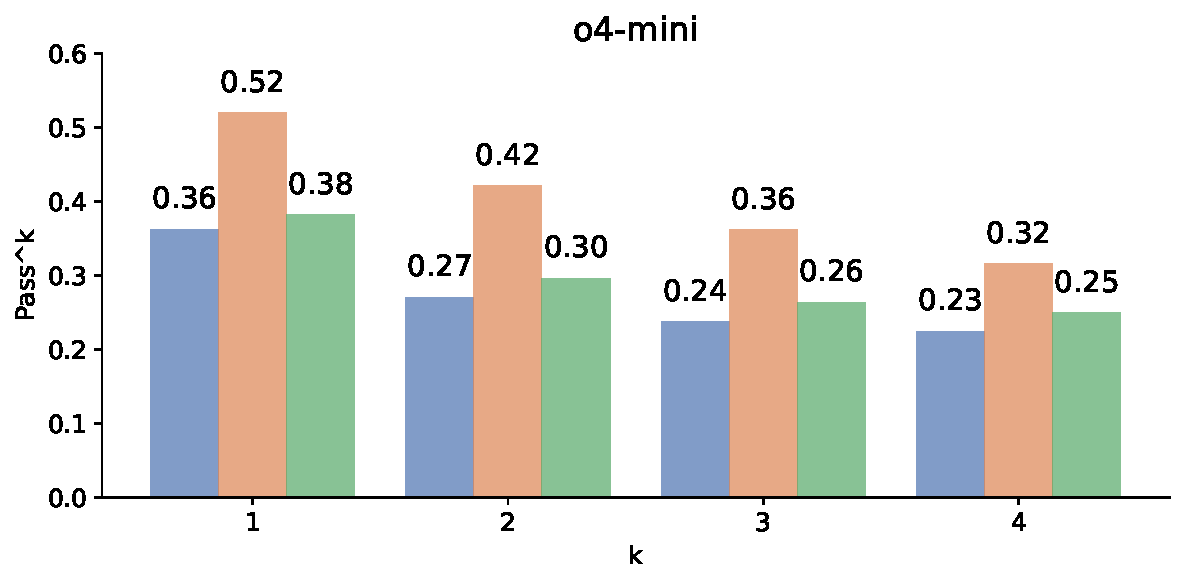
\includegraphics[width=\textwidth]{figures/results/pass_k_vs_k_per_persona_telecom_o4-mini-2025-04-16.pdf}
    \end{subfigure}
    \vspace{0.5em}
    \begin{subfigure}[tb]{0.48\textwidth}
        \centering
        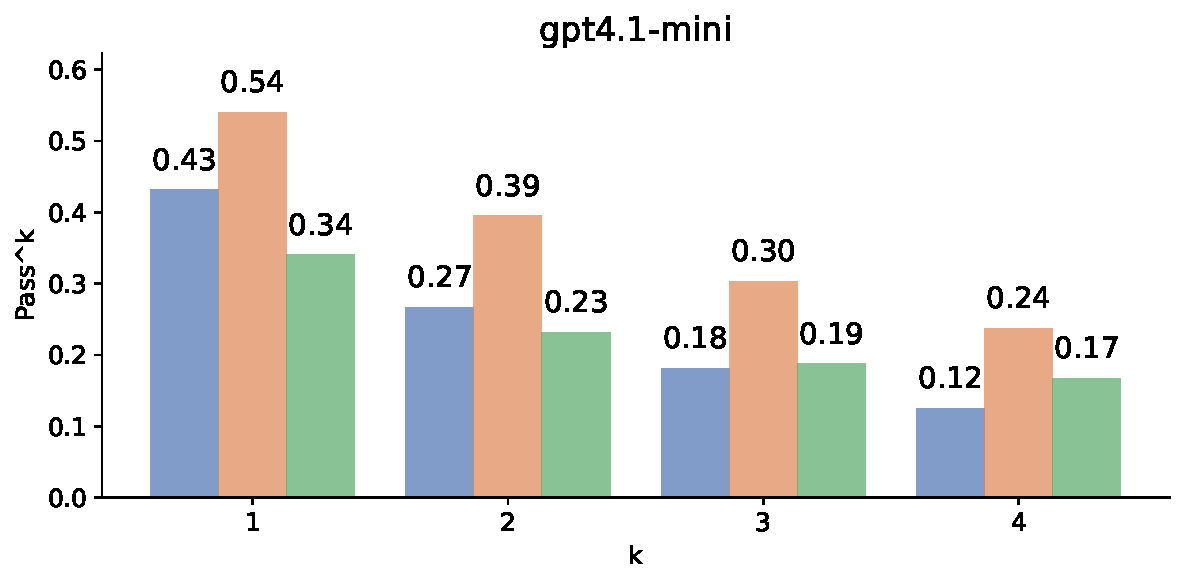
\includegraphics[width=\textwidth]{figures/results/pass_k_vs_k_per_persona_telecom_gpt-4.1-mini-2025-04-14.pdf}
    \end{subfigure}
    \hfill
    \begin{subfigure}[tb]{0.48\textwidth}
        \centering
        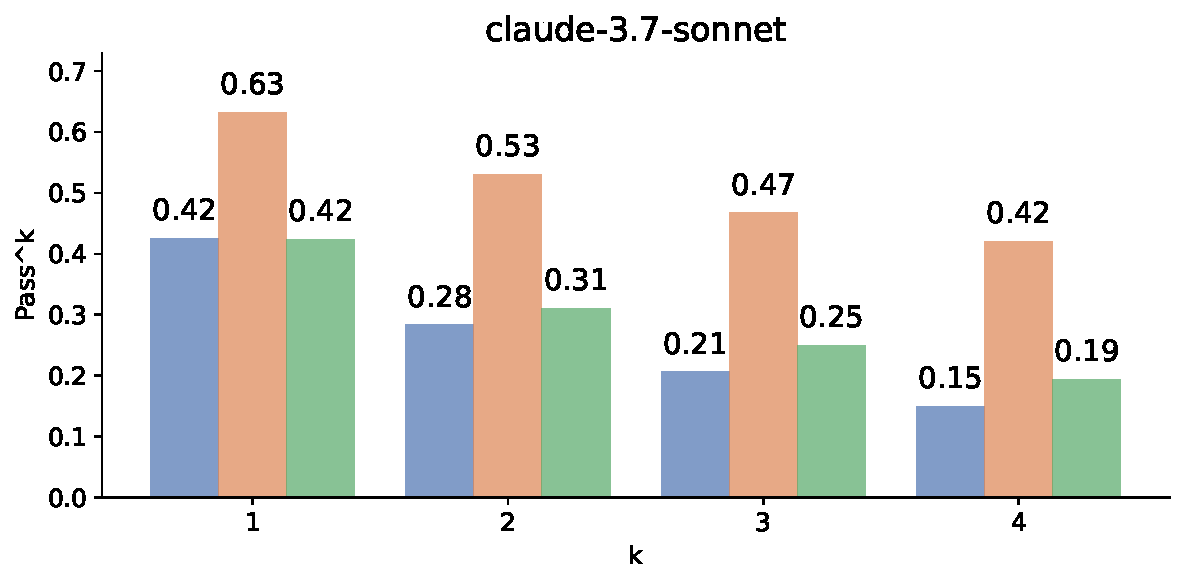
\includegraphics[width=\textwidth]{figures/results/pass_k_vs_k_per_persona_telecom_claude-3-7-sonnet-20250219.pdf}
    \end{subfigure}
    \vspace{-0.8em}
    \caption{\gptmodelshort (top left), \ofourmodelshort (top right), \gptminishort (bottom left), and \claudesonnetshort (bottom right) \passk per persona type for the \telecom domain. Performance is shown across different persona types, highlighting how different user characteristics affect success rates.}
    \label{fig:telecom_persona_results}
    \vspace{-1em}
\end{figure} 


\textbf{Impact of user persona.}
\Cref{fig:telecom_persona_results} provides an breakdown analysis of performance by user persona.
Results confirm that the agent tends to perform better on tasks associated with the \texttt{Easy} persona compared to those associated with the \texttt{Hard} one. Interestingly, the performances of the agent on tasks involving no persona information (\texttt{None}) tend to be be on par or lower to performances on tasks associated with the \texttt{Hard} persona. This highlights the critical importance of testing AI systems with well-defined user personas before real-world deployment.
\subsection{How does dual-control impact benchmark reliability?}
\label{sec:reliability}

Ensuring the reliability of conversational agent benchmarks is paramount. Three primary sources of uncertainty can impact benchmark reliability: \textbf{implementation errors}, \textbf{task specification errors}, and \textbf{user simulator errors}. While the user simulator is often cited as a critical component requiring careful evaluation, its assessment can be confounded by issues in the benchmark's implementation or task definitions. Therefore, we first address these potential error sources before evaluating the user simulator itself. This is detailed in \Cref{app:verify_tau}.

\paragraph{User simulator quality evaluation.}

Having minimized errors in the benchmark implementation and task specifications, we evaluated the user simulator quality.

To assess the quality of the user simulator across domains, we manually annotated interaction traces generated using \gptmodelshort for both the User Simulator and the Agent.

Each conversation was reviewed by two separate annotators tasked with identifying user simulator errors. 
Annotators were given the User Simulator Guidelines, the specific User Instructions for this conversation (see \Cref{app:user-prompt}), descriptions of the available User Tools (if any), and the complete conversation trajectory (messages and tool calls). Annotators assessed each user turn against four criteria: adherence to \textbf{User Simulator Guidelines}, adherence to \textbf{User Instructions}, correct use of \textbf{User Tools}, and generation of a \textbf{natural and consistent} conversational continuation.

Errors were categorized as either (1) \textbf{task‑critical} errors: high‑severity failures that preclude task completion (e.g., generating an intent that contradicts the user goal, or causing an irrecoverable state transition),  or as (2) \textbf{task‑benign} errors: Errors that do not prevent the task from being completed.



\paragraph{Reliability of the user simulator.}
\label{sec:user-sim-quality}

\begin{table}[tbp]
    \centering
    \caption{User simulator error count (\textit{rates}) across domains. Only critical user errors prevent the agent from solving the task while benign errors do not affect task completion. New \telecom domain shows much lower error rate and no critical errors were reported. (See \Cref{app:user-sim-quality} for additional details).}
    \label{tab:user_sim_error_rates}
    \vspace{0.2em}
    \begin{adjustbox}{width=0.8\linewidth}
    \begin{tabular}{l|l|l|l|l}
        \toprule
        \textbf{Domain} & \textbf{Num Conversations} & \textbf{Critical Errors} & \textbf{Benign Errors} & \textbf{Total Errors}\\
        \midrule
        \airline & 100  & 13 (\textit{13\%}) & 34 (\textit{34\%}) & 47 (\textit{47\%})\\
        \retail & 50  & 6 (\textit{12\%}) & 14 (\textit{28\%})& 20 (\textit{40\%}) \\
        \telecom & 50  & 3 (\textit{6\%}) & 5 (\textit{10\%}) & 8 (\textit{16\%})\\
        \bottomrule
    \end{tabular}
    \end{adjustbox}
    \vspace{-0.5em}
\end{table}




As shown in \Cref{tab:user_sim_error_rates}, our analysis of user simulator behavior reveals significant improvements in reliability for the new \telecom domain. While for the \retail and \airline domains we recorded a 40\% and 47\% error rate for the user simulator (with 12\% and 13\% being critical errors that prevent task completion), this rate is much lower for the \telecom domain, only 16\% with 6\% critical errors reported. This substantial improvement in reliability can be attributed to the domain design, which shapes and tightly constrains user behavior through its environment and available affordances. Rather than relying heavily on natural language specifications to guide behavior, the \telecom domain's structured interface and clear action space naturally guide the user simulator toward correct interactions, resulting in more consistent and predictable behavior.

